\subsection{Работа с файлами}
\begin{frame}[fragile]
	\frametitle{Чтение байт из файла}

	\begin{Large}
	\begin{minted}[bgcolor=bgcode]{java}
	FileInputStream fis;
	byte [] buf = new byte[10];

	fis = new FileInputStream("1.txt");
	fis.read(buf);
	\end{minted}
	\end{Large}
\end{frame}

\begin{frame}[fragile]
	\frametitle{Чтение символов}

	\begin{columns}[c]
	\column{2.8in}
	\begin{minted}[bgcolor=bgcode]{java}
	FileInputStream fis;
	InputStreamReader is;
	char [] buf = new char[10];

	fis = new FileInputStream("1.txt");
	is = new InputStreamReader(
	                    is, "utf-8");

	is.read(buf);
	\end{minted}
	\column{1.7in}
	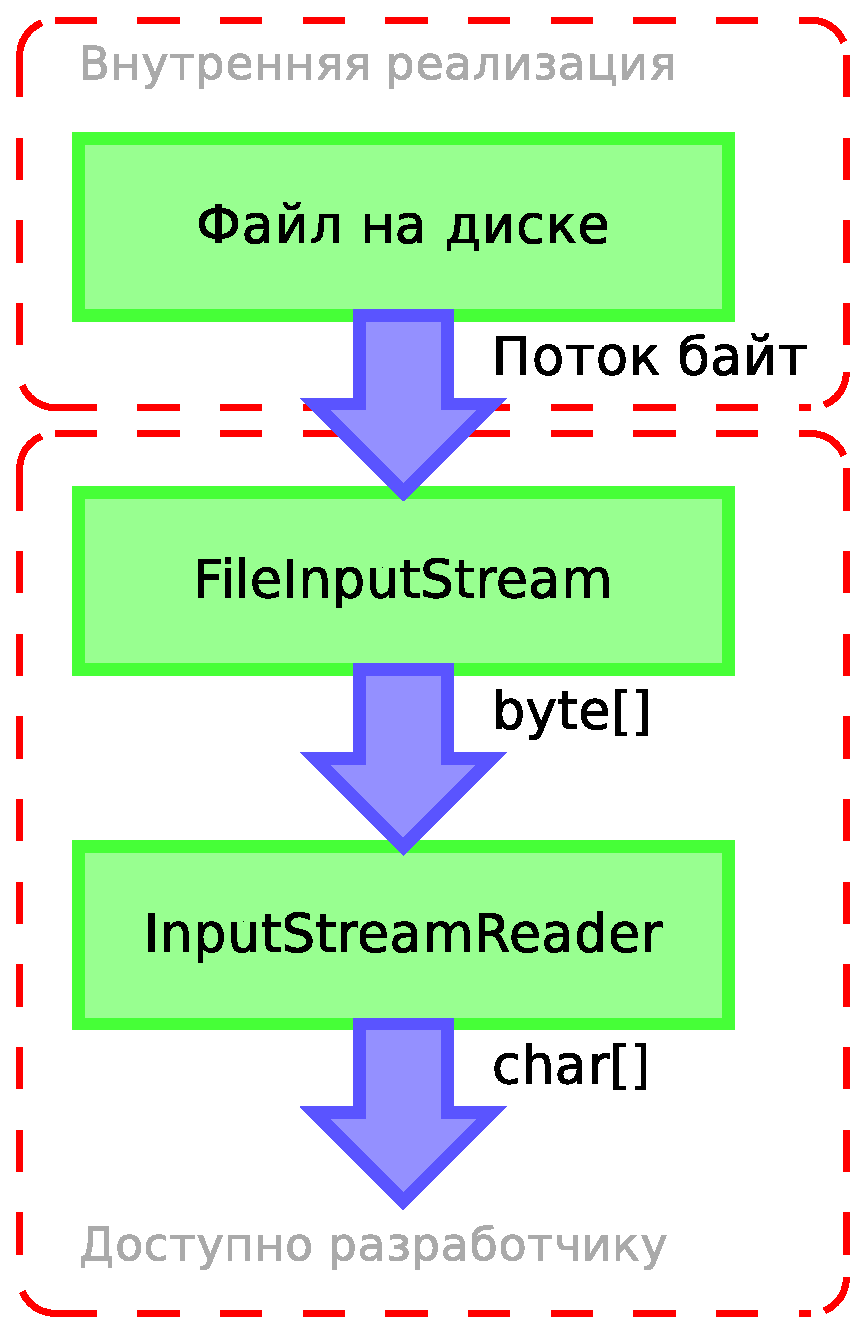
\includegraphics[width=1.75in]{lesson-3-Diagram1.eps}
	\end{columns}
\end{frame}

\begin{frame}[fragile]
	\frametitle{FileReader -- объединение FileInputStream и InputStreamReader для удобства}

	\begin{Large}
	
	\begin{minted}[bgcolor=bgcode]{java}
	FileReader fr;
	char [] buf = new char[10];

	fr = new FileReader("1.txt");
	fr.read(buf);
	\end{minted}
	\end{Large}
\end{frame}


\section{Наследование}

\subsection{Наследование атрибутов}
\begin{frame}[fragile]
	\frametitle{Наследование -- одно из свойств ООП}

	\begin{columns}[c]
	\column{2.3in}
	\begin{Large}
	Наследование -- механизм, позволяющий описать новый класс на основе уже существующего.
	\end{Large}
	\bigskip

	\begin{large}
	При этом объекты нового класса будут обладать всеми свойствами родительского класса. Вообще говоря они даже будут принадлежать базовому классу.
	\end{large}
	\column{2.15in}
	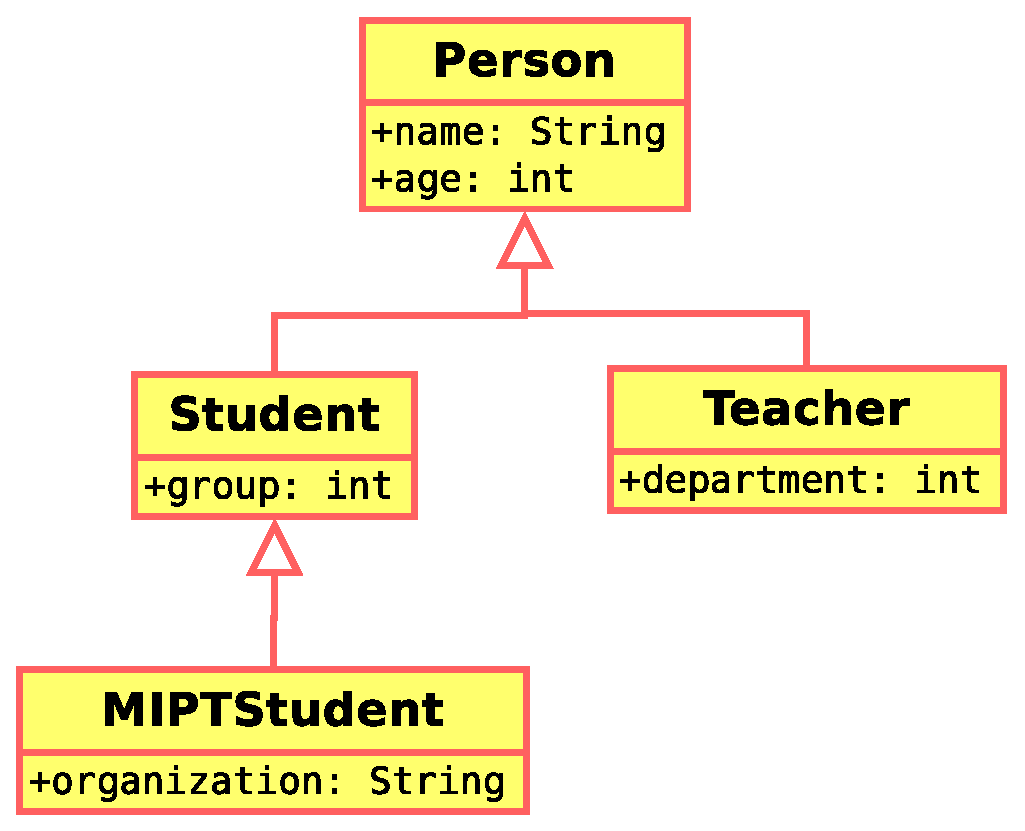
\includegraphics[width=2.2in]{lesson-4-Diagram1.eps}
	\end{columns}
\end{frame}

\begin{frame}
	\frametitle{Отношения между объектами}

	\begin{columns}[c]
	\column{2.8in}
	\begin{large}
	\begin{itemize}
	\item{Каждый \emph{Student} является \emph{Person}ом.}
	\item{Каждый \emph{MIPTStudent} является как \emph{Student}ом так и \emph{Person}ом.}
	\item{\emph{Person} может быть \emph{Student}ом, \emph{MIPTStudent}ом, \emph{Teacher}ом, а может и не быть.}
	\item{\emph{MIPTStudent} будет иметь все аттрибуты \emph{Student}а и \emph{Person}а, а также свои: name, age, group, organization.}
	\end{itemize}
	\end{large}
	\column{1.65in}
	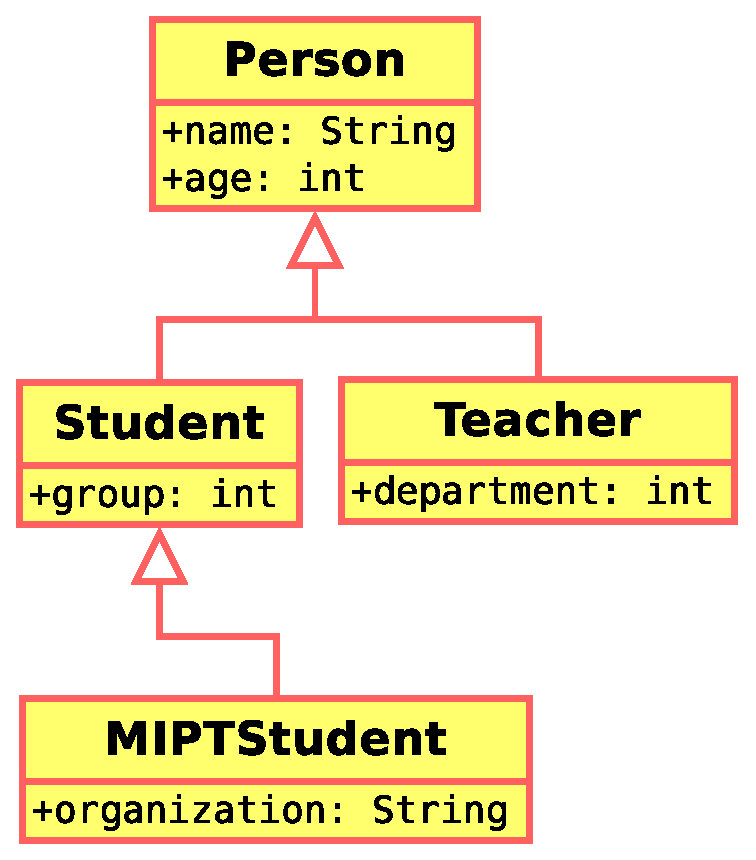
\includegraphics[width=1.7in]{lesson-4-Diagram2.eps}
	\end{columns}
\end{frame}

\begin{frame}
	\frametitle{Термины}

	\begin{figure}[H]
	\centering
	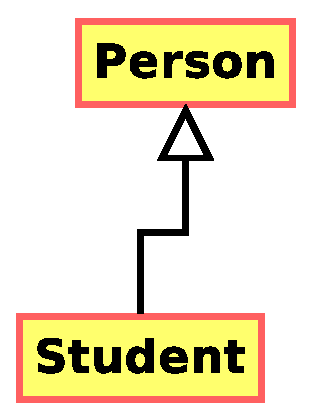
\includegraphics[width=1in]{lesson-4-Diagram3.eps}
	\end{figure}

	\begin{itemize}
	\item{Класс \emph{Person} -- базовый, родительский, суперкласс (base, parent, superclass) по отношению к \emph{Student}}
	\item{Класс \emph{Student} -- дочерний, подкласс (extended, derived, child, subclass) по отношению к \emph{Person}}
	\end{itemize}
\end{frame}

\begin{frame}[fragile]
	\frametitle{Напишем код классов Person и Student}

	\begin{minted}[bgcolor=bgcode,linenos=true,baselinestretch=0.9]{java}
	class Person {
	    String name;
	    int age;
	}

	class Student extends Person {
	    int group;
	}
	
	class App {
	    public static void main(String [] args) {
	        Student s = new Student();

	        s.name = "Ivanov Ivan";
	        s.age = 18;

	        s.group = 234;
	    }
	}
	\end{minted}
\end{frame}

\begin{frame}[fragile]
	\frametitle{Ссылки на объект другого класса}

	\begin{large}
	\begin{minted}[bgcolor=bgcode]{java}
	Student s = new Student();
	Person p = s;
	\end{minted}
	\end{large}
	\color{gray}
	-- так делать можно, потому что \emph{Student} является \emph{Person}ом. Однако используя ссылку \emph{p} можно получить доступ только к полям, определенным в классе \emph{Person}.

	\medskip
	Cделать обратное присваивание немного сложнее:
	\color{black}
	\begin{large}
	\begin{minted}[bgcolor=bgcode]{java}
	Student s2 = (Student)p;
	\end{minted}
	\end{large}

	\color{gray}
	При таком присваивании во время выполнения программы проверяется его корректность, например при выполнении кода
	\color{black}
	\begin{large}
	\begin{minted}[bgcolor=bgcode]{java}
	Teacher t = (Teacher)p;
	\end{minted}
	\end{large}
	\color{gray}
	возникнет ошибка \emph{ClassCastException}.
	\color{black}
\end{frame}

\begin{frame}[fragile]
	\frametitle{Класс Object}

	\begin{columns}[c]
	\column{2.0in}
	\begin{Large}
	Все классы в Java неявно наследуются от класса \emph{Object}.
	\end{Large}
	\bigskip

	\column{2.45in}
	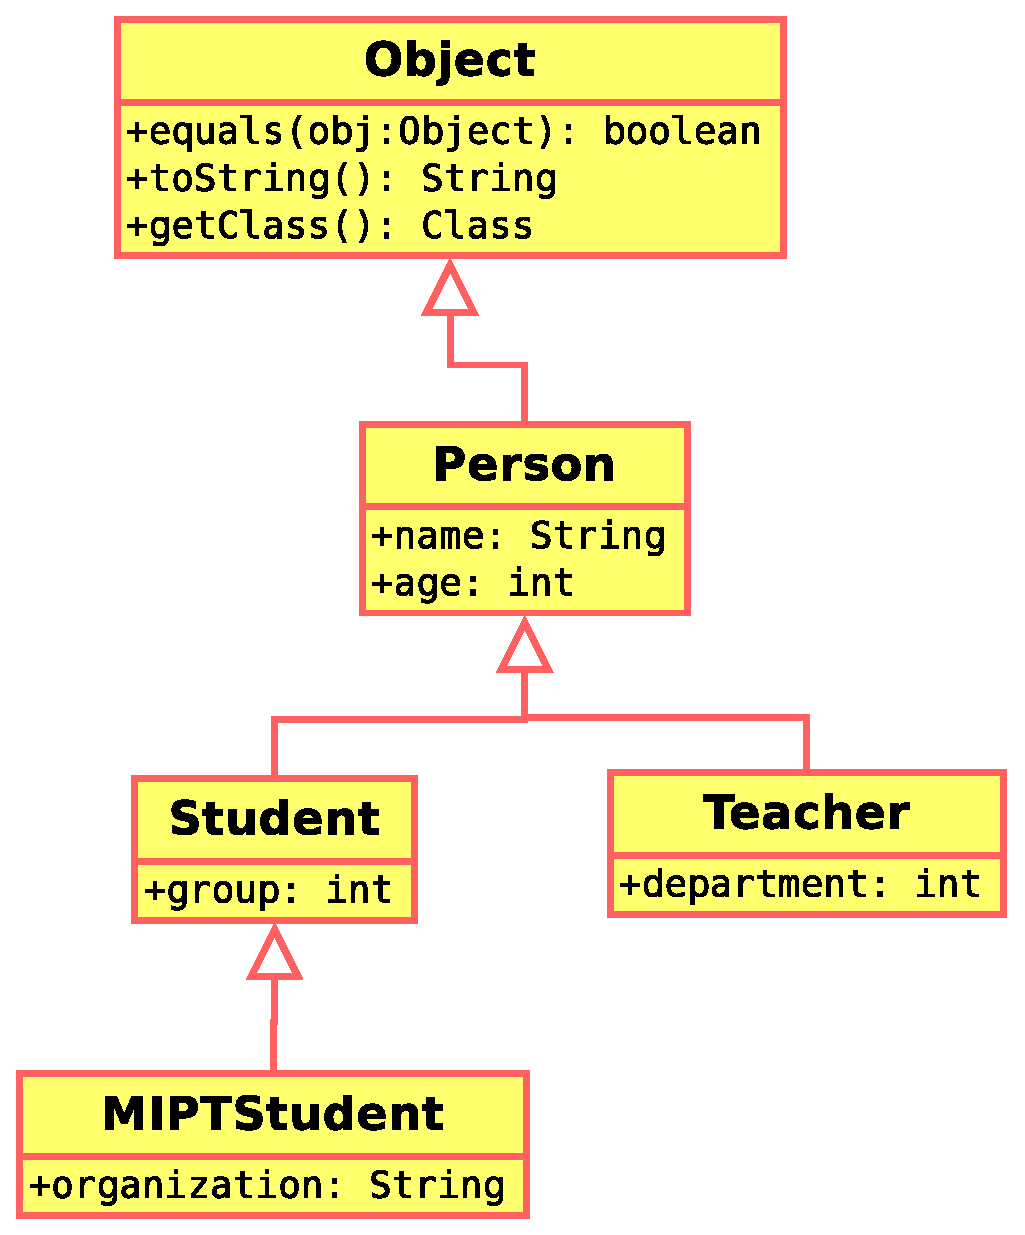
\includegraphics[width=2.5in]{lesson-4-Diagram4.eps}
	\end{columns}
\end{frame}


\subsection{Переопределение методов}
\begin{frame}[fragile]
	\frametitle{Переопределение методов}

	\begin{minted}[bgcolor=bgcode,linenos=true,baselinestretch=0.8]{java}
	class Parent {
	    int x = 10;
	    void print() {
	        System.out.println("I'm a parent");
	    }
	}
	class Child extends Parent {
	    String x = "qwe";
	    void print() {
	        System.out.println("I'm a child");
	    }
	}
	class App {
	    public static void main(String [] args) {
	        Parent p = new Child();
	        System.out.println(p.x); /* 10 */
	        p.print(); /* I'm a child */
	    }
	}
	\end{minted}
\end{frame}

\begin{frame}
	\frametitle{Пример использования}

	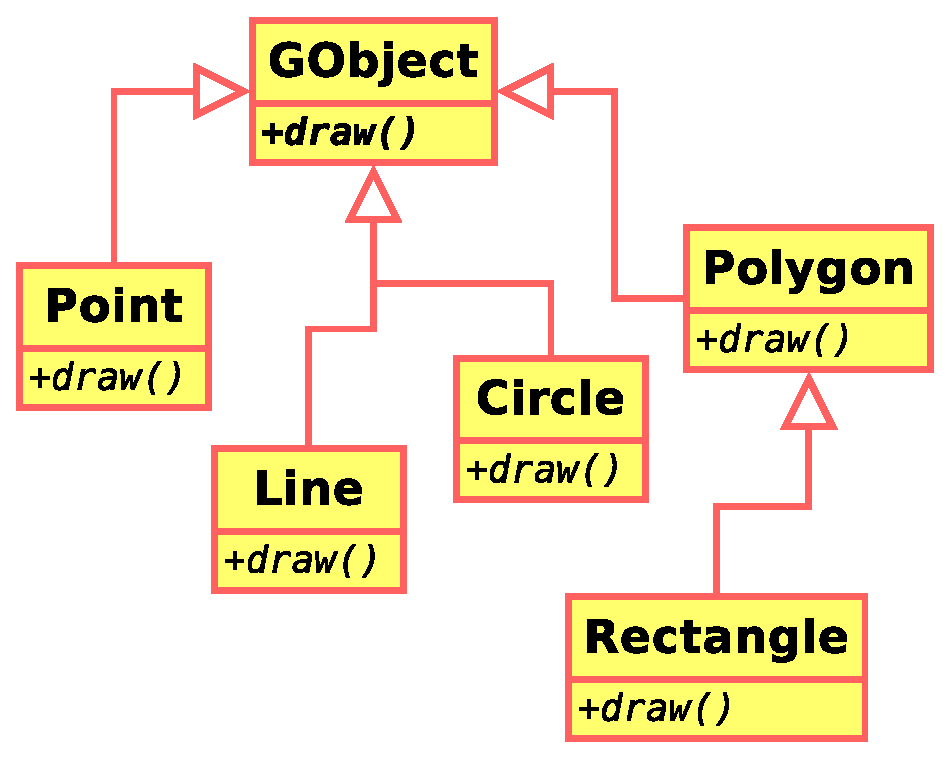
\includegraphics[width=0.9\linewidth]{lesson-4-Diagram5.eps}
\end{frame}

\begin{frame}[fragile]
	\frametitle{Пример использования}

	\begin{large}
	\begin{minted}[bgcolor=bgcode,linenos=true]{java}
	GObject arr[] = new GObject[5];

	arr[0] = new Point();
	arr[1] = new Line();
	arr[2] = new Circle();
	arr[3] = new Polygon();
	arr[4] = new Rectangle();

	for(i = 0; i < arr.length; i++)
	    arr[i].draw();
	\end{minted}
	\end{large}
\end{frame}

\begin{frame}
	\frametitle{Пример из стандартной библиотеки}

	\begin{Large}
	\begin{itemize}
	\item{Есть классы, которые производят поток байт: \emph{FileInputStream}, \emph{PipedInputStream}, \emph{DeflaterInputStream}}
	\item{Имеется класс, который может перевести текст из любой кодировки в UNICODE: \emph{InputStreamReader}}
	\end{itemize}

	Как сделать так, чтобы можно было читать поток символов UNICODE из любого объекта классов \emph{FileInputStream}, \emph{PipedInputStream}, \emph{DeflaterInputStream} ?
	\end{Large}
\end{frame}

\begin{frame}[fragile]
	\frametitle{Пример из стандартной библиотеки}

	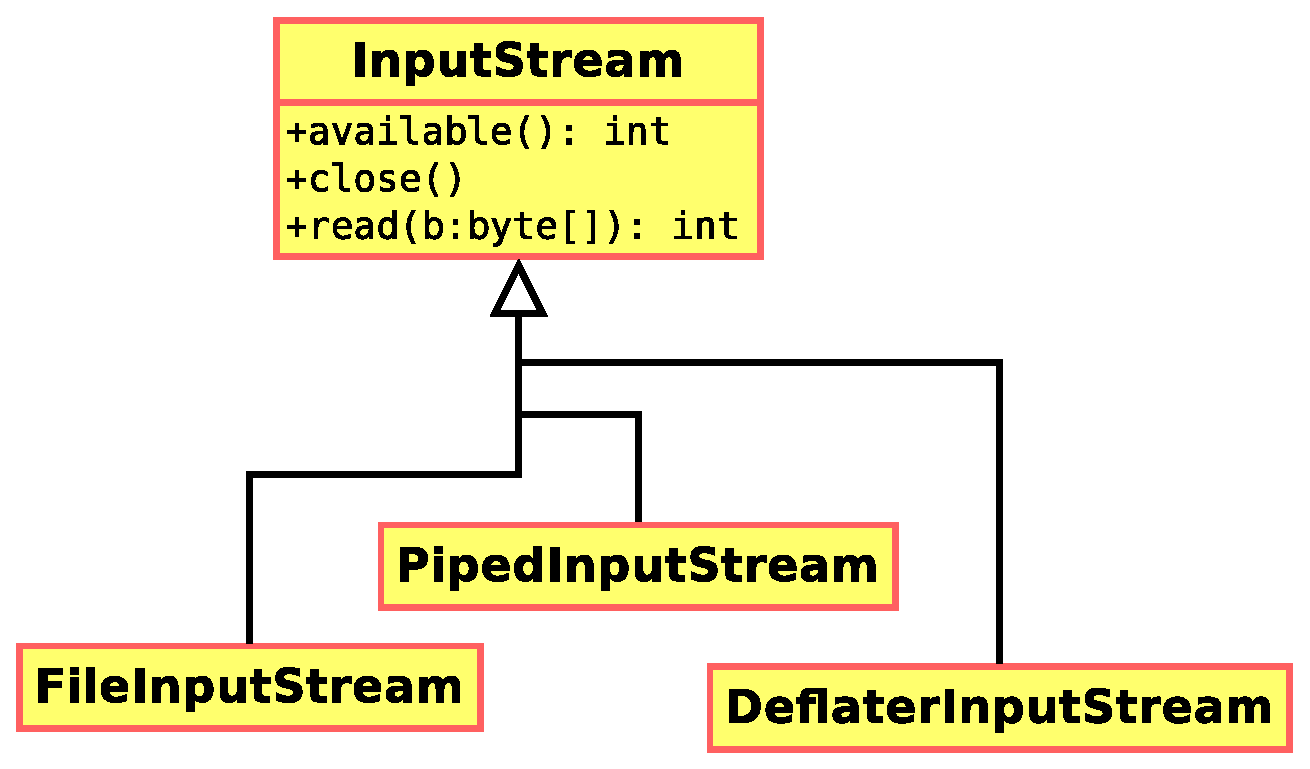
\includegraphics[height=0.6\textheight]{lesson-4-Diagram6.eps}

	\medskip
	\begin{minted}[bgcolor=bgcode,linenos=true,baselinestretch=0.8]{java}
	class InputStreamReader {
	    InputStreamReader(InputStream stream) {
	        ...
	\end{minted}
\end{frame}

\begin{frame}[fragile]
	\frametitle{Конструкторы не наследуются !}

	\begin{large}
	Надо явно вызывать конструктор базового класса, если это необходимо.
	\medskip
	\begin{minted}[bgcolor=bgcode,linenos=true,baselinestretch=0.8]{java}
	class MyClass1 {
	    int x;
	    MyClass1(int x) {
	        this.x = x;
	    }
	}

	class MyClass2 extends MyClass1 {
	    int y;
	    MyClass2(int x, int y) {
	        super(x);

	        this.y = y;
	    }
	}
	\end{minted}
	\end{large}

\end{frame}

\subsection{Ключевое слово final}
\begin{frame}
	\frametitle{Ключевое слово final}

	\begin{Large}
	Имеет разное значение, в зависимости от того, к чему применяется
	\medskip
	\begin{itemize}
	\item{\emph{Поле} -- присвоить значение этому полю можно только один раз.}
	\item{\emph{Метод} -- нельзя переопределить}
	\item{\emph{Класс} -- от него ничего нельзя унаследовать}
	\end{itemize}
	\end{Large}
\end{frame}

\subsection{Задачи}
\begin{frame}[fragile]
	\frametitle{Задачи}
	\begin{small}
	\begin{enumerate}
	\parindent 5mm
		\begin{item}
		Сделать метод \texttt{printTable(Function f, float start, float step, int n);}, который печатает таблицу значений функции. Функция -- объект класс Function, имеет метод \texttt{float get(float(x));}.
		
		Сделать 2 дочерних класса, например, для линейной функции и параболы, в которых будет переопределен метод \texttt{get}.
		
		Продемонстрировать работу метода: cделать класс Function с методом для печати в консоль таблицы значений в заданном диапазоне, который использует метод get (пустой в классе Function) и сделать 2 подкласса: линейная функция и парабола, которые будут переопределять метод \texttt{get}.

		\begin{minted}[bgcolor=bgcode,linenos=true,baselinestretch=0.8]{java}
			Parabola p = new Parabola(1, 2, 3);
			Line l = new Line(2, 5);

			printTable(p, 0, 0.1, 20);
			printTable(l, 0, 0.1, 20);
		\end{minted}
		\end{item}
	\end{enumerate}
	\end{small}
\end{frame}
